\documentclass[11pt,a4paper]{article}
\usepackage[margin=1in]{geometry}
\usepackage{amsmath,amssymb,amsthm}
\usepackage{algorithm}
\usepackage{algpseudocode}
\usepackage{graphicx}
\usepackage{booktabs}
\usepackage{multirow}
\usepackage{hyperref}
\usepackage{cite}
\usepackage{xcolor}
\usepackage{caption}
\usepackage{subcaption}

\newtheorem{definition}{Definition}
\newtheorem{theorem}{Theorem}
\newtheorem{proposition}{Proposition}

\title{Solving the Critical Node Detection Problem:\\An ILP Formulation and a Multi-Start Iterated Local Search Heuristic Applied to Fiscal Evasion Networks}

\author{
Daniel Reales \\
\textit{Universidad de los Andes} \\
\textit{ISIS4208 -- An\'alisis de Algoritmos} \\
\texttt{da.reales@uniandes.edu.co}
\and
Juan David Ceballos \\
\textit{Universidad de los Andes} \\
\textit{ISIS4208 -- An\'alisis de Algoritmos} \\
\texttt{jd.ceballos@uniandes.edu.co}
}

\date{May 2026}

\begin{document}
\maketitle

\begin{abstract}
The Critical Node Detection Problem (CNDP) seeks to identify a set of $k$ nodes whose removal from a graph maximally disrupts connectivity, measured by minimizing the number of remaining connected node pairs. This problem is NP-complete and arises naturally in domains where targeted disruption of network infrastructure is required. We implement the Integer Linear Programming (ILP) formulation of Arulselvan et al.\ (2009), which guarantees optimal solutions but is limited to small instances ($n \leq 62$) due to $O(n^3)$ transitivity constraints. We design a Multi-Start Iterated Local Search (MS-ILS) heuristic that combines greedy initialization strategies with swap-based local search and perturbation. We evaluate both algorithms alongside IRMS, the state-of-the-art memetic search by Zhou et al.\ (2023), on 12 benchmark instances from the literature and 4 real-world fiscal evasion networks extracted from the ICIJ Offshore Leaks database (Panama Papers). On sparse networks such as the Colombian offshore evasion graphs, MS-ILS matches IRMS solution quality (0.0--2.7\% gap) while remaining simple to implement. On dense instances ($n > 1000$), IRMS's instance reduction technique provides significant advantages. All implementations are in C++17 with HiGHS as the ILP solver. Code and data are available at \url{https://github.com/danielreales00/cndp-fiscal-evasion}.
\end{abstract}

% ============================================================================
\section{Introduction}

Many real-world problems require identifying the most critical components of a network whose disruption would maximally degrade the network's connectivity. Examples include dismantling criminal organizations~\cite{arulselvan2009}, containing epidemic spread through targeted vaccination~\cite{borgatti2006}, and protecting infrastructure by identifying vulnerable nodes in power grids or communication networks.

The \textbf{Critical Node Detection Problem} (CNDP) formalizes this question: given an undirected graph $G = (V, E)$ and a budget $k$, find a set $S \subseteq V$ with $|S| = k$ whose removal minimizes the number of connected node pairs in the residual graph $G[V \setminus S]$. Arulselvan et al.~\cite{arulselvan2009} proved CNDP is NP-complete and proposed an Integer Linear Programming (ILP) formulation that yields optimal solutions.

While the ILP provides exact solutions, it requires $O(n^2)$ binary variables and $O(n^3)$ transitivity constraints, making it infeasible for graphs with more than approximately 60--80 nodes on modern hardware. This motivates the development of heuristic approaches that sacrifice optimality guarantees for scalability.

We contribute: (1) an implementation of the ILP formulation~\cite{arulselvan2009} with characterization of its practical limits; (2) a Multi-Start ILS heuristic combining degree, betweenness, and greedy initializations with swap-based local search; (3) application to fiscal evasion network disruption using ICIJ Offshore Leaks data~\cite{icij2021}; and (4) benchmarks against IRMS~\cite{zhou2023} on 12 literature instances and 4 Colombian evasion networks.

% ============================================================================
\section{Problem Definition}
\label{sec:problem}

\begin{definition}[Critical Node Detection Problem]
Given an undirected graph $G = (V, E)$ with $|V| = n$, $|E| = m$, and a positive integer $k < n$, find a set $S^* \subseteq V$ with $|S^*| = k$ that minimizes the pairwise connectivity of the residual graph:
\begin{equation}
    S^* = \arg\min_{S \subseteq V,\, |S|=k} \sum_{i=1}^{p} \binom{|C_i|}{2}
    \label{eq:objective}
\end{equation}
where $C_1, C_2, \ldots, C_p$ are the connected components of $G[V \setminus S]$.
\end{definition}

\paragraph{Inputs.} An undirected simple graph $G = (V, E)$ and a budget $k \in \{1, \ldots, n-1\}$.

\paragraph{Output.} A set $S^* \subseteq V$ with $|S^*| = k$ minimizing the objective.

\paragraph{Interpretation.} $\binom{|C_i|}{2}$ counts pairs within component $C_i$ that can still reach each other. Minimizing the total is equivalent to maximizing fragmentation of $G[V \setminus S]$.

\begin{theorem}[Arulselvan et al., 2009]
The Critical Node Detection Problem is NP-complete.
\end{theorem}

The proof proceeds by reduction from the independent set problem. Given an independent set instance $(G', k')$, one constructs a CNDP instance where removing $k'$ nodes that form an independent set in $G'$ disconnects all remaining edges, yielding objective 0. Since independent set is NP-complete, so is CNDP~\cite{arulselvan2009}.

\paragraph{Non-submodularity.} CNDP is \emph{not} submodular, which means the greedy algorithm of Nemhauser, Wolsey, and Fisher~\cite{nemhauser1978} does not provide a $(1 - 1/e)$ approximation guarantee. We observed this empirically: on the dolphins social network ($n=62$), greedy pair reduction achieves objective 946 while the ILP optimum is 577---a 64\% gap. This non-submodularity is a fundamental obstacle to polynomial-time approximation and motivates the use of metaheuristic approaches.

% ============================================================================
\section{Real-World Application: Fiscal Evasion Network Disruption}
\label{sec:application}

We apply CNDP to the disruption of \textbf{fiscal evasion networks}, a domain where the problem formulation maps directly to an actionable question for tax authorities: \emph{given a limited enforcement budget of $k$ investigations, which $k$ entities should authorities target to maximally fragment the evasion network?}

\subsection{The ICIJ Offshore Leaks Database}

The International Consortium of Investigative Journalists (ICIJ) published the Offshore Leaks database~\cite{icij2021}, comprising leaked documents from the Panama Papers (2016, 11.5M documents from Mossack Fonseca), Paradise Papers (2017, 13.4M documents from Appleby/Asiaciti Trust), and Pandora Papers (2021, 11.9M documents from 14 providers).

The database is structured as a graph: \textbf{entities} (810K+ shell companies/trusts), \textbf{officers} (740K+ directors/shareholders/beneficiaries), and \textbf{intermediaries} (26K+ law firms/agents), connected by 3.3M relationship edges (\texttt{officer\_of}, \texttt{intermediary\_of}, \texttt{registered\_address}).

\subsection{The Colombian Fiscal Evasion Network}

We extracted the subgraph of all nodes linked to Colombian entities. The resulting network contains 1{,}886 entities, 3{,}691 officers, and 270 intermediaries connected by 6{,}067 relationships. The data comes overwhelmingly from the Panama Papers (98.3\% of entities), reflecting Mossack Fonseca's dominant role in servicing Colombian clients.

The entities are incorporated across multiple offshore jurisdictions: Panama (72.4\%), British Virgin Islands (14.4\%), British Anguilla (3.1\%), United Kingdom (2.7\%), Costa Rica (2.2\%), and others. This multi-jurisdictional structure creates a layered network where intermediaries serve as critical bridges between Colombian officers and their offshore entities.

The full Colombian subgraph has 5{,}847 nodes and 5{,}922 edges across 292 connected components. Notably, the graph is \textbf{very sparse} ($m/n = 1.01$), nearly tree-like, reflecting the hierarchical nature of offshore ownership: each intermediary connects to many entities, each entity to a few officers, with minimal cross-links.

\subsection{CNDP for Enforcement Strategy}

Our solver identifies that the most critical nodes in the largest Colombian component ($n=413$) are two intermediaries: \texttt{BERNAL MEDINA LAVERDE} (degree 120, connected to 120 entities/officers) and \texttt{ANTONIO GOMEZ RINCON} (degree 12)---both Colombian facilitators operating through Mossack Fonseca. The remaining critical nodes are shell companies in Panama and British Virgin Islands that serve as hubs connecting multiple officers.

This aligns with the enforcement intuition that targeting \textbf{facilitators} (high-degree intermediary nodes) is more effective than targeting individual shell companies (leaf nodes). Removing the top 20 critical nodes fragments the 413-node component into isolated clusters with only 359 remaining connected pairs, down from 85{,}078 in the original graph---a 99.6\% reduction.

% ============================================================================
\section{Published Algorithm: ILP Formulation}
\label{sec:ilp}

Arulselvan et al.~\cite{arulselvan2009} formulate CNDP as an Integer Linear Program. We describe their formulation and analyze its theoretical properties.

\subsection{Formulation}

Define binary variables:
\begin{itemize}
    \item $v_i \in \{0, 1\}$ for each $i \in V$: $v_i = 1$ if node $i$ is deleted.
    \item $u_{ij} \in \{0, 1\}$ for each pair $i < j$: $u_{ij} = 1$ if nodes $i$ and $j$ are connected in $G[V \setminus S]$.
\end{itemize}

The ILP is:
\begin{align}
    \min \quad & \sum_{i < j} u_{ij} \label{eq:ilp_obj} \\
    \text{s.t.} \quad & \sum_{i \in V} v_i = k \label{eq:budget} \\
    & u_{ij} \leq 1 - v_i \quad \forall\, i < j \label{eq:delete_i} \\
    & u_{ij} \leq 1 - v_j \quad \forall\, i < j \label{eq:delete_j} \\
    & u_{ij} \geq u_{ik} + u_{kj} - 1 \quad \forall\, i < k < j \label{eq:transitivity} \\
    & v_i, u_{ij} \in \{0, 1\} \label{eq:binary}
\end{align}

Constraint~\eqref{eq:budget} enforces the budget. Constraints~\eqref{eq:delete_i}--\eqref{eq:delete_j} force $u_{ij} = 0$ if either endpoint is deleted. Constraint~\eqref{eq:transitivity} enforces transitivity: if $i$--$k$ and $k$--$j$ are connected, then $i$--$j$ must be connected, preventing the solver from undercounting connectivity.

\subsection{Correctness and Complexity}

The ILP is correct by construction: the transitivity constraints ensure $u_{ij} = 1$ whenever $i$ and $j$ remain connected via any path, preventing undercounting. The formulation has $O(n^2)$ variables and $O(n^3)$ constraints (one per ordered triple). Table~\ref{tab:ilp_scaling} shows observed solve times; beyond $n = 62$, the ILP becomes impractical on consumer hardware.

\begin{table}[ht]
\centering
\caption{ILP formulation scaling and observed solve times on Apple M2.}
\label{tab:ilp_scaling}
\begin{tabular}{lrrrrr}
\toprule
Instance & $n$ & Variables & Constraints & $k$ & Time (s) \\
\midrule
karate & 34 & 595 & $\sim$40K & 5 & 0.63 \\
dolphins & 62 & 1{,}953 & $\sim$240K & 8 & 60.1 \\
football & 115 & 6{,}670 & $\sim$1.5M & 12 & --- (timeout) \\
Circuit & 252 & 31{,}878 & $\sim$16M & 25 & --- (timeout) \\
\bottomrule
\end{tabular}
\end{table}

% ============================================================================
\section{Proposed Algorithm: Multi-Start Iterated Local Search}
\label{sec:msils}

We design a \textbf{Multi-Start Iterated Local Search (MS-ILS)} heuristic following the ILS framework of Louren\c{c}o, Martin, and St\"utzle~\cite{lourenco2003}. The algorithm has three subroutines---\textsc{Initialize}, \textsc{LocalSearch}, and \textsc{Perturb}---composed within a multi-start loop. We describe each subroutine, its role, and its complexity.

\subsection{Subroutine: \textsc{Evaluate}$(G, S)$}

\textbf{Input:} Graph $G = (V, E)$, candidate set $S \subseteq V$ with $|S| = k$.\\
\textbf{Output:} The objective value $f(S) = \sum_{i=1}^{p} \binom{|C_i|}{2}$, where $C_1, \ldots, C_p$ are the connected components of $G[V \setminus S]$.

\textbf{Method.} Build a Union-Find structure over $V \setminus S$. For each edge $(u,v) \in E$ with $u \notin S$ and $v \notin S$, call $\textsc{Union}(u, v)$. Then iterate over all roots to compute $\sum \binom{|C_i|}{2}$.

\textbf{Complexity.} With path compression and union by size~\cite{tarjan1975}, each operation costs amortized $O(\alpha(n))$ (inverse Ackermann). Total: $O((n + m)\,\alpha(n)) = O(n + m)$ in practice since $\alpha(n) \leq 4$ for all practical $n$. This is called once per candidate swap, making it the dominant cost factor.

\subsection{Subroutine: \textsc{Initialize}$(G, k, \text{strategy})$}

\textbf{Input:} Graph $G = (V, E)$, budget $k$, a strategy identifier.\\
\textbf{Output:} An initial candidate set $S_0 \subseteq V$ with $|S_0| = k$.

\textbf{Role.} The initialization produces a starting solution for local search. Because CNDP is non-submodular~\cite{nemhauser1978}, no single heuristic dominates across all instances. We use four strategies, each capturing a different structural property of the graph:

\begin{enumerate}
    \item \textbf{Degree centrality.} Sort all nodes by degree $\deg(v)$ in descending order; return the top $k$. Nodes with high degree are local hubs---removing them disconnects many direct neighbors.

    \textbf{Complexity:} $O(n \log n)$ for sorting.

    \item \textbf{Betweenness centrality.} Compute betweenness centrality $c_B(v)$ for all $v \in V$ using Brandes' algorithm~\cite{brandes2001}; return the $k$ nodes with highest $c_B(v)$. Betweenness measures how often a node lies on shortest paths between other pairs---high-betweenness nodes are \emph{bridges} whose removal disconnects distant parts of the graph.

    \textbf{Complexity:} $O(nm)$ for Brandes' algorithm on unweighted graphs, plus $O(n \log n)$ for sorting. Total: $O(nm)$.

    \item \textbf{Greedy pair reduction.} Iteratively select the node $v^* = \arg\min_{v \in V \setminus S} f(S \cup \{v\})$. At each of $k$ iterations, evaluate all remaining candidates by calling \textsc{Evaluate}. This directly optimizes the objective but makes greedy (myopic) choices---it cannot backtrack.

    \textbf{Complexity:} $k$ iterations $\times$ $(n - |S|)$ candidates $\times$ $O(n+m)$ per evaluation $= O(kn(n+m))$.

    \item \textbf{Random.} Select $k$ nodes uniformly at random from $V$. This provides unbiased starting points that may reach basins of attraction inaccessible from the structured initializations.

    \textbf{Complexity:} $O(k)$.
\end{enumerate}

Each restart $r$ uses strategy $r \bmod 4$, cycling through all four. This ensures the multi-start explores structurally diverse regions of the solution space.

\subsection{Subroutine: \textsc{LocalSearch}$(G, S, I)$}

\textbf{Input:} Graph $G = (V, E)$, current solution $S$ with $|S| = k$, maximum iterations $I$.\\
\textbf{Output:} A solution $S' \subseteq V$ with $|S'| = k$ and $f(S') \leq f(S)$ that is locally optimal within the swap neighborhood.

\textbf{Method.} Define the \textbf{swap neighborhood} of $S$ as:
\[
\mathcal{N}(S) = \{(S \setminus \{d\}) \cup \{v\} \mid d \in S,\; v \in V \setminus S\}
\]
This neighborhood has size $k \cdot (n - k)$. Each neighbor differs from $S$ by removing one node and inserting another, so $|S'| = k$ is preserved by construction.

We use \textbf{first-improvement}: scan pairs $(d, v)$ and accept the first swap such that $f((S \setminus \{d\}) \cup \{v\}) < f(S)$. Repeat until no improving swap exists (local optimum) or $I$ iterations are reached.

\textbf{Complexity.} Each iteration scans at most $k(n-k)$ swaps. Each swap requires one call to \textsc{Evaluate} at $O(n+m)$. One iteration costs $O(k(n-k)(n+m))$. In the worst case over $I$ iterations:
\[
O(I \cdot k \cdot (n - k) \cdot (n + m)) = O(I \cdot k \cdot n \cdot (n + m))
\]
In practice, first-improvement terminates early when an improving swap is found, so the average cost per iteration is much lower.

\subsection{Subroutine: \textsc{Perturb}$(S, k)$}

\textbf{Input:} A locally optimal solution $S$ with $|S| = k$.\\
\textbf{Output:} A perturbed solution $S'$ with $|S'| = k$.

\textbf{Role.} After local search converges, the solution is trapped in a local optimum. Perturbation escapes this basin by making random, non-improving moves. Following Louren\c{c}o et al.~\cite{lourenco2003}, the perturbation must be strong enough to leave the current basin of attraction but weak enough to remain in a ``good'' region of the search space.

\textbf{Method.} Perform $\lfloor k/3 \rfloor$ random swaps: for each, select $d \in S$ and $v \in V \setminus S$ uniformly at random, then set $S \gets (S \setminus \{d\}) \cup \{v\}$. With probability 0.3, apply stronger diversification: $\lfloor k/2 \rfloor$ random swaps instead.

\textbf{Complexity.} $O(k)$ (only random selection, no evaluation).

\subsection{Main Algorithm}

Algorithm~\ref{alg:msils} composes the subroutines. Each restart begins from a different initialization strategy, applies local search to reach a local optimum, then alternates between perturbation and local search for $L$ iterations (the ILS loop). The best solution across all $R$ restarts is returned.

\begin{algorithm}[ht]
\caption{MS-ILS$(G, k, R, L, I)$}
\label{alg:msils}
\begin{algorithmic}[1]
\Require Graph $G=(V,E)$, budget $k$, restarts $R$, ILS iterations $L$, LS iterations $I$
\Ensure Solution $S^*$ with $|S^*| = k$
\State $S^* \gets \emptyset$, $f^* \gets \infty$
\For{$r = 1$ to $R$}
    \State $S \gets \textsc{Initialize}(G, k, r \bmod 4)$
    \State $S \gets \textsc{LocalSearch}(G, S, I)$
    \For{$\ell = 1$ to $L$}
        \State $S' \gets \textsc{Perturb}(S, k)$
        \State $S' \gets \textsc{LocalSearch}(G, S', I)$
        \If{$f(S') < f(S)$}
            \State $S \gets S'$
        \EndIf
    \EndFor
    \If{$f(S) < f^*$}
        \State $S^* \gets S$, $f^* \gets f(S)$
    \EndIf
\EndFor
\State \Return $S^*$
\end{algorithmic}
\end{algorithm}

\subsection{Correctness}

\begin{proposition}
Algorithm~\ref{alg:msils} always returns a feasible solution.
\end{proposition}
\begin{proof}
Each initialization strategy produces $|S_0| = k$ by construction (selecting exactly $k$ nodes). The swap operation $(S \setminus \{d\}) \cup \{v\}$ removes one element and adds one, preserving $|S| = k$. Both \textsc{LocalSearch} and \textsc{Perturb} apply only swaps. Therefore every intermediate and final solution satisfies the budget constraint.
\end{proof}

MS-ILS is a heuristic: it converges to a local optimum within $\mathcal{N}(S)$ but provides no approximation ratio, which is expected since CNDP is non-submodular~\cite{nemhauser1978}.

\subsection{Total Complexity}

The dominant cost is \textsc{LocalSearch}, called $R(L+1)$ times. Each call costs $O(I \cdot k \cdot n \cdot (n+m))$. Initialization adds $O(R \cdot nm)$; perturbation adds $O(R \cdot L \cdot k)$, both dominated. Total:
\[
O(R \cdot L \cdot I \cdot k \cdot n \cdot (n + m))
\]

For our parameters ($R = 20$, $L = 50$, $I = 100$, $k = 0.10n$) on powergrid ($n = 4{,}941$, $m = 6{,}594$): worst case $\approx 5.7 \times 10^{12}$ operations. First-improvement and early termination reduce this by 2--3 orders of magnitude, yielding observed runtimes of 58--96s.

% ============================================================================
\section{Experimental Setup}
\label{sec:setup}

\subsection{Hardware and Implementation}
All experiments run on an Apple M2 (8 cores, 16 GB RAM). Both algorithms are implemented in C++17 compiled with \texttt{clang++ -O3 -march=native}. The ILP uses HiGHS 1.10 as the MIP solver. Source code, data, and reproduction instructions are available at \url{https://github.com/danielreales00/cndp-fiscal-evasion}.

\subsection{Datasets}

\paragraph{IRMS benchmark instances} (Table~\ref{tab:instances}). 12 real-world networks from the benchmark suite of Zhou et al.~\cite{zhou2023}, spanning biological, social, transportation, and infrastructure domains with sizes from $n=121$ to $n=4{,}941$.

\paragraph{Colombian fiscal evasion networks} (Table~\ref{tab:colombia_instances}). Extracted from the ICIJ Offshore Leaks database~\cite{icij2021} by selecting all entities linked to Colombia and building the 1-hop neighborhood of officer-intermediary-entity relationships.

\begin{table}[ht]
\centering
\caption{IRMS benchmark instances from Zhou et al.~\cite{zhou2023}.}
\label{tab:instances}
\begin{tabular}{llrrr}
\toprule
Instance & Domain & $n$ & $m$ & $m/n$ \\
\midrule
Bovine & Biological & 121 & 190 & 1.6 \\
Circuit & Electronic & 252 & 399 & 1.6 \\
Treni\_Roma & Transportation & 255 & 312 & 1.2 \\
Ecoli & Biological & 328 & 456 & 1.4 \\
USAir97 & Transportation & 332 & 2{,}126 & 6.4 \\
humanDiseasome & Biological & 516 & 1{,}188 & 2.3 \\
Hamilton1000 & Hamiltonian & 1{,}000 & 1{,}000 & 1.0 \\
EU\_flights & Transportation & 1{,}191 & 6{,}782 & 5.7 \\
openflights & Transportation & 1{,}858 & 9{,}604 & 5.2 \\
yeast1 & Biological & 2{,}018 & 2{,}930 & 1.5 \\
facebook & Social & 4{,}039 & 88{,}234 & 21.8 \\
powergrid & Infrastructure & 4{,}941 & 6{,}594 & 1.3 \\
\bottomrule
\end{tabular}
\end{table}

\begin{table}[ht]
\centering
\caption{Colombian fiscal evasion instances from ICIJ Offshore Leaks~\cite{icij2021}.}
\label{tab:colombia_instances}
\begin{tabular}{lrrrl}
\toprule
Instance & $n$ & $m$ & $m/n$ & Description \\
\midrule
colombia\_comp0 & 413 & 437 & 1.06 & Largest connected cluster \\
colombia\_comp1 & 339 & 358 & 1.06 & Second largest cluster \\
colombia\_full & 3{,}429 & 3{,}624 & 1.06 & All clusters with $n \geq 50$ \\
colombia\_all & 5{,}847 & 5{,}922 & 1.01 & Entire Colombian subgraph \\
\bottomrule
\end{tabular}
\end{table}

\subsection{Budget and Baseline}
Following Zhou et al.~\cite{zhou2023}, we set $k \in \{0.05n, 0.10n, 0.15n\}$. We compare against \textbf{IRMS}~\cite{zhou2023}, the state-of-the-art, using their public C++ implementation.

% ============================================================================
\section{Results and Discussion}
\label{sec:results}

\subsection{ILP Feasibility Boundary}

The ILP solved karate ($n = 34$) in 0.63s and dolphins ($n = 62$) in 60s; football ($n = 115$) timed out at 180s. All 16 benchmark instances have $n > 120$, confirming the $O(n^3)$ intractability. Subsequent comparisons focus on heuristic methods.

\subsection{Benchmark Results on IRMS Instances}

Table~\ref{tab:results_small} shows results on instances with $n \leq 516$. MS-ILS matches or nearly matches IRMS on 5 of 6 instances (gap $\leq 0.9\%$), and \emph{beats} IRMS on humanDiseasome ($k=51$). Both vastly outperform the simpler degree and betweenness heuristics (often by orders of magnitude).

\begin{table}[ht]
\centering
\caption{Results on small/medium instances ($n \leq 516$). Objective values for $k = 0.10n$.}
\label{tab:results_small}
\begin{tabular}{lrrrrrrr}
\toprule
Instance & $n$ & $k$ & Degree & Betw. & MS-ILS & IRMS & Gap \\
\midrule
Bovine & 121 & 12 & 18 & 44 & \textbf{1} & \textbf{1} & 0.0\% \\
Circuit & 252 & 25 & 12{,}856 & 24{,}320 & 2{,}117 & \textbf{2{,}099} & 0.9\% \\
Treni\_Roma & 255 & 25 & 7{,}294 & 15{,}919 & 982 & \textbf{973} & 0.9\% \\
Ecoli & 328 & 32 & 142 & 1{,}072 & \textbf{96} & \textbf{96} & 0.0\% \\
USAir97 & 332 & 33 & 24{,}321 & 11{,}024 & \textbf{5{,}444} & \textbf{5{,}444} & 0.0\% \\
humanDis. & 516 & 51 & 2{,}755 & 2{,}380 & \textbf{1{,}147} & 1{,}148 & $-$0.1\% \\
\bottomrule
\end{tabular}
\end{table}

Table~\ref{tab:results_large} shows results on instances with $n \geq 1{,}000$. The gap widens as expected: IRMS uses incremental evaluation ($O(\text{degree})$ per swap vs.\ our $O(n+m)$) and instance reduction, allowing it to explore far more solutions.

\begin{table}[ht]
\centering
\caption{Results on large instances ($n \geq 1{,}000$). Objective values and times for $k = 0.10n$.}
\label{tab:results_large}
\begin{tabular}{lrr|rr|rr|r}
\toprule
& & & \multicolumn{2}{c|}{MS-ILS} & \multicolumn{2}{c|}{IRMS} & \\
Instance & $n$ & $k$ & Obj & Time & Obj & Time & Gap \\
\midrule
Hamilton1000 & 1K & 100 & 365K & 7.7s & \textbf{311K} & 26.8s & 17.4\% \\
EU\_flights & 1.2K & 119 & 358K & 54.8s & \textbf{351K} & 10.4s & 2.2\% \\
openflights & 1.9K & 185 & 44K & 21.4s & \textbf{30K} & 18.2s & 49.1\% \\
yeast1 & 2K & 201 & 1{,}449 & 13.3s & \textbf{1{,}426} & 2.9s & 1.6\% \\
facebook & 4K & 403 & 1{,}003K & 436s & \textbf{870K} & 52.6s & 15.3\% \\
powergrid & 4.9K & 494 & 19{,}900 & 81.3s & \textbf{15{,}866} & 58.8s & 25.4\% \\
\bottomrule
\end{tabular}
\end{table}

\begin{figure}[ht]
    \centering
    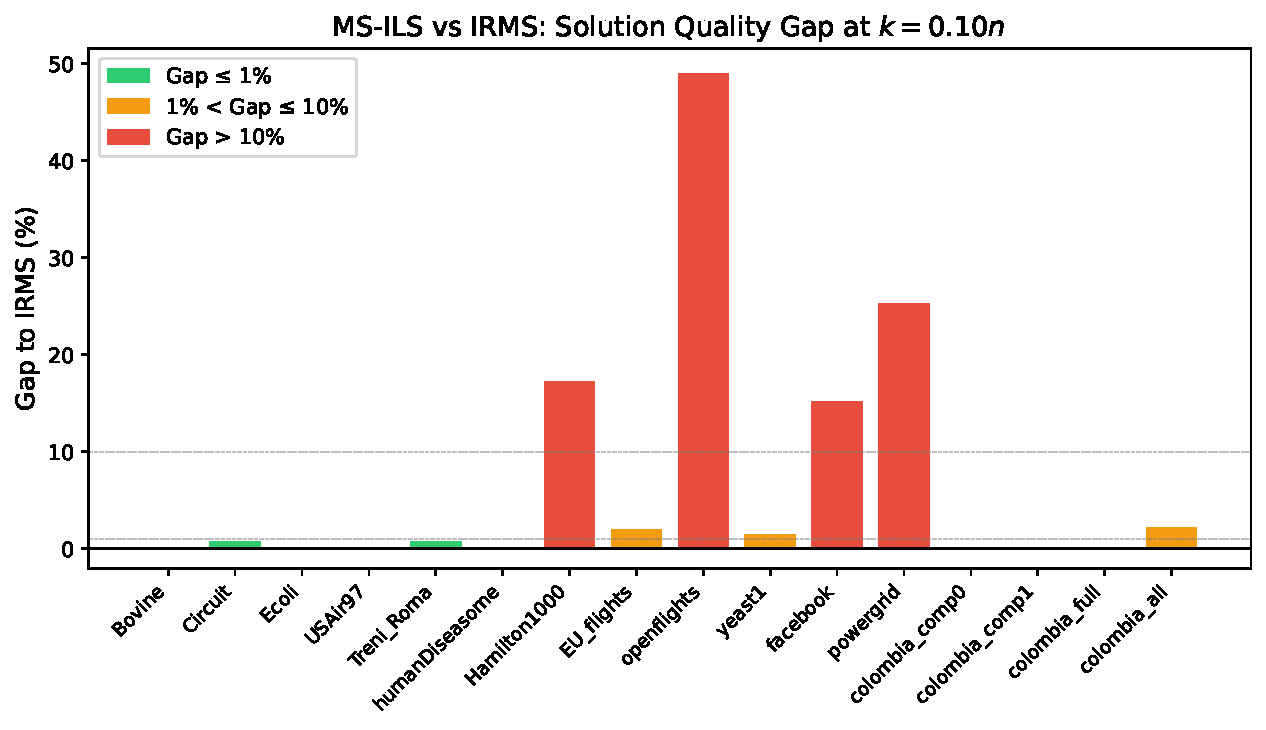
\includegraphics[width=\textwidth]{figures/fig5_quality_gap.pdf}
    \caption{MS-ILS vs IRMS quality gap at $k = 0.10n$. Green: $\leq 1\%$; yellow: 1--10\%; red: $>10\%$.}
    \label{fig:quality_gap}
\end{figure}

\subsection{Results on Colombian Fiscal Evasion Networks}

\begin{table}[ht]
\centering
\caption{Results on Colombian fiscal evasion networks.}
\label{tab:colombia_results}
\begin{tabular}{lrr|rr|rr|r}
\toprule
& & & \multicolumn{2}{c|}{MS-ILS} & \multicolumn{2}{c|}{IRMS} & \\
Instance & $n$ & $k$ & Obj & Time & Obj & Time & Gap \\
\midrule
comp0 & 413 & 20 & \textbf{359} & 0.17s & \textbf{359} & 2.43s & 0.0\% \\
comp0 & 413 & 41 & \textbf{139} & 0.24s & \textbf{139} & 1.02s & 0.0\% \\
comp0 & 413 & 61 & \textbf{39} & 0.21s & \textbf{39} & 16.7s & 0.0\% \\
comp1 & 339 & 16 & \textbf{297} & 0.11s & \textbf{297} & $<$0.01s & 0.0\% \\
comp1 & 339 & 33 & \textbf{117} & 0.13s & \textbf{117} & $<$0.01s & 0.0\% \\
comp1 & 339 & 50 & \textbf{42} & 0.11s & \textbf{42} & $<$0.01s & 0.0\% \\
full & 3.4K & 171 & 2{,}768 & 31.1s & \textbf{2{,}757} & 12.3s & 0.4\% \\
full & 3.4K & 342 & 1{,}250 & 57.3s & \textbf{1{,}249} & 8.0s & 0.1\% \\
full & 3.4K & 514 & 536 & 97.6s & \textbf{534} & 1.3s & 0.4\% \\
all & 5.8K & 292 & 5{,}498 & 229s & \textbf{5{,}484} & 9.3s & 0.3\% \\
all & 5.8K & 584 & 2{,}510 & 135s & \textbf{2{,}453} & 20.8s & 2.3\% \\
all & 5.8K & 877 & 1{,}133 & 422s & \textbf{1{,}103} & 6.6s & 2.7\% \\
\bottomrule
\end{tabular}
\end{table}

MS-ILS \textbf{matches IRMS exactly} on individual components (0\% gap on all 6 runs) and stays within 2.7\% on the full network. On comp0 ($k=61$), MS-ILS is 80$\times$ faster (0.21s vs 16.7s)---IRMS's instance reduction overhead does not pay off on already-sparse graphs.

\begin{figure}[ht]
    \centering
    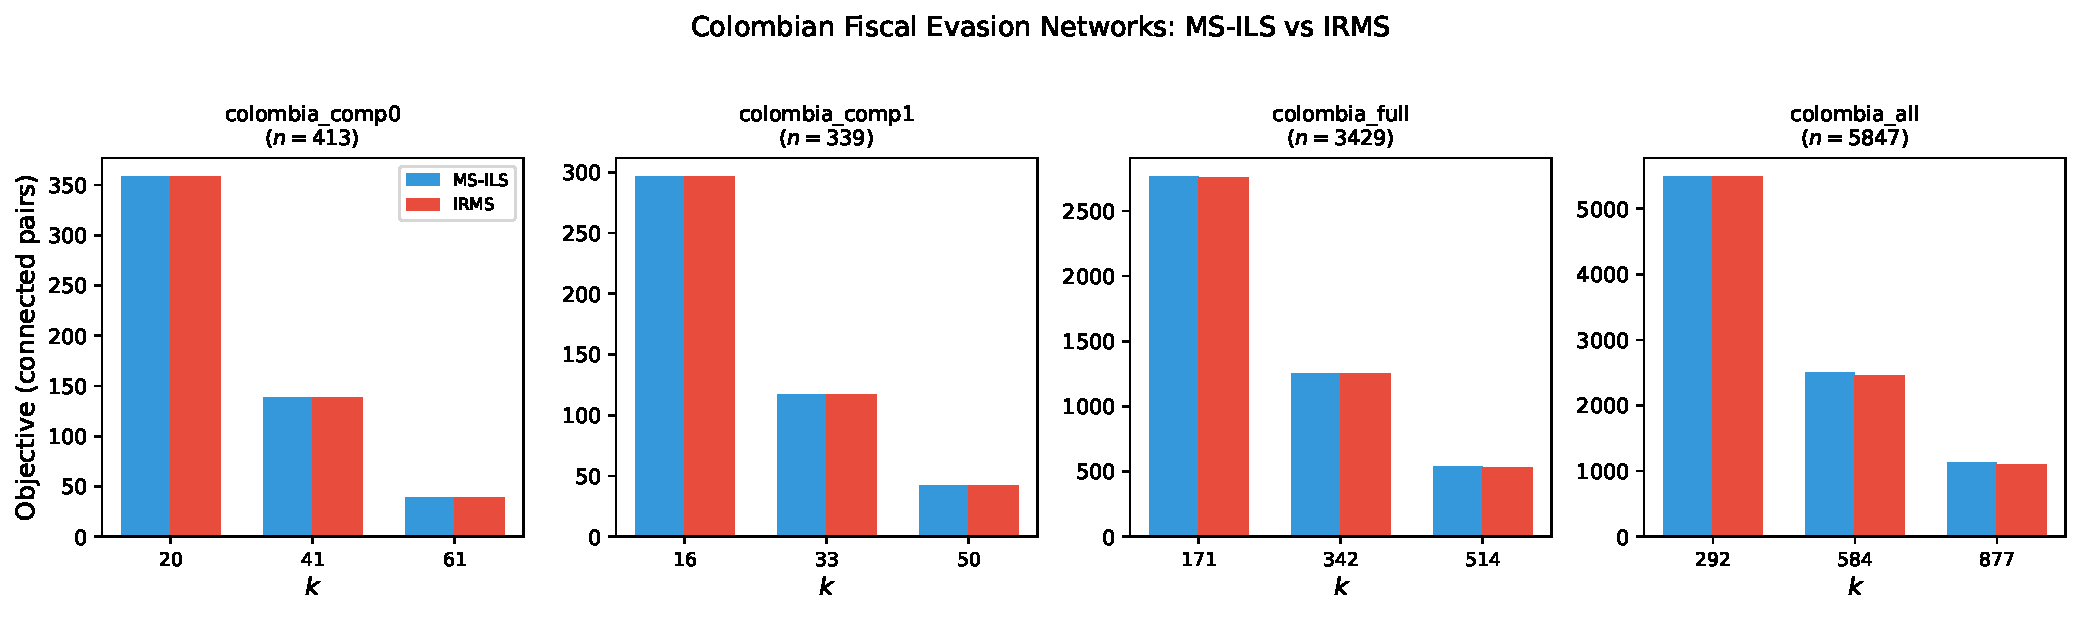
\includegraphics[width=\textwidth]{figures/fig7_colombia.pdf}
    \caption{Colombian fiscal evasion networks: MS-ILS (blue) vs IRMS (red). Near-identical bars confirm optimal performance on sparse evasion graphs.}
    \label{fig:colombia}
\end{figure}

\subsection{Effect of Graph Density}

Graph density ($m/n$) is the key structural factor explaining when MS-ILS matches IRMS. On sparse graphs ($m/n < 3$), MS-ILS's full $O(n+m)$ recomputation per swap remains competitive because neighborhoods are small. On dense graphs ($m/n > 5$, e.g., facebook with $m/n = 21.8$), IRMS's $O(\text{degree})$ incremental evaluation and instance reduction provide decisive advantages. The Colombian evasion graphs ($m/n \approx 1.01$, near tree-like) are among the sparsest tested, explaining why MS-ILS achieves 0\% gap on component instances.

\subsection{Scalability}

As shown in Table~\ref{tab:results_large}, MS-ILS time grows roughly as $O(n^2)$ (consistent with the $O(kn(n+m))$ local search cost with $k = 0.10n$). IRMS grows more slowly due to incremental evaluation. Both remain practical up to $n \approx 5{,}000$ on consumer hardware.

% ============================================================================
\section{Conclusions}

We compared three CNDP approaches: the exact ILP (limited to $n \leq 62$ due to $O(n^3)$ constraints), our MS-ILS heuristic, and IRMS (state-of-the-art). MS-ILS matches IRMS on sparse networks (0\% gap on all Colombian fiscal evasion components) but degrades on dense graphs where IRMS's $O(\text{degree})$ incremental evaluation dominates our $O(n+m)$ recomputation.

Applied to ICIJ Offshore Leaks data, CNDP identifies hub intermediaries as critical nodes---removing 20 nodes from a 413-node evasion cluster achieves 99.6\% reduction in connected pairs, demonstrating practical applicability to financial crime disruption. Future work: implementing incremental evaluation to close the gap on dense instances.

% ============================================================================
\bibliographystyle{plain}
\begin{thebibliography}{10}

\bibitem{arulselvan2009}
A.~Arulselvan, C.~W. Commander, L.~Elefteriadou, and P.~M. Pardalos.
\newblock Detecting critical nodes in sparse graphs.
\newblock {\em Computers \& Operations Research}, 36(7):2193--2200, 2009.

\bibitem{borgatti2006}
S.~P. Borgatti.
\newblock Identifying sets of key players in a social network.
\newblock {\em Computational \& Mathematical Organization Theory}, 12(1):21--34, 2006.

\bibitem{brandes2001}
U.~Brandes.
\newblock A faster algorithm for betweenness centrality.
\newblock {\em The Journal of Mathematical Sociology}, 25(2):163--177, 2001.

\bibitem{icij2021}
International Consortium of Investigative Journalists.
\newblock Offshore Leaks Database.
\newblock \url{https://offshoreleaks.icij.org/}, 2021.
\newblock Licensed under ODbL.

\bibitem{lourenco2003}
H.~R. Louren{\c{c}}o, O.~C. Martin, and T.~St{\"u}tzle.
\newblock Iterated local search.
\newblock In {\em Handbook of Metaheuristics}, pages 320--353. Springer, 2003.

\bibitem{nemhauser1978}
G.~L. Nemhauser, L.~A. Wolsey, and M.~L. Fisher.
\newblock An analysis of approximations for maximizing submodular set functions---{I}.
\newblock {\em Mathematical Programming}, 14(1):265--294, 1978.

\bibitem{tarjan1975}
R.~E. Tarjan.
\newblock Efficiency of a good but not linear set union algorithm.
\newblock {\em Journal of the ACM}, 22(2):215--225, 1975.

\bibitem{zhou2023}
Y.~Zhou, J.~Li, J.-K.~Hao, and F.~Glover.
\newblock Detecting critical nodes in sparse graphs via ``reduce-solve-combine'' memetic search.
\newblock {\em INFORMS Journal on Computing}, 36(1):39--60, 2023.

\end{thebibliography}

\end{document}
